\chapter{Ingeniería Inversa} \label{cap:capitulo3}

En este capítulo se procede a documentar el proceso de ingeniería inversa al que se ha sometido a limitador que puede verse en la imagen {imagen}.

Tal y como se comentó en la sección \ref{sec:contexto}, el punto de partida del proyecto es el estudio y análisis de un limitador funcional y operativo que se encuentra en el laboratorio de \gls{granasat}. Es importante recordar que se dispone del código fuente de este limitador, así como su manual de usuario, el cual nos será de gran ayuda para poder instalarlo correctamente y conocer las capacidades y características generales del producto. De aquí en adelante, se hará referencia al este limitador como \acrshort{LM7}, ya que ese es el nombre técnico del producto.

!! IMAGEN DE LIMITADOR
\label{img:lms7_cls}

\section{Instalación del limitador}

El primer paso a realizar para comenzar el proceso de ingeniería inversa es instalar el equipo. Para ello, se recurre al manual de usuario del equipo, y se siguen las instrucciones de instalación. En la figura \ref{fig:lm7_montaje} se puede observar el esquema de montaje del limitador en un entorno objetivo, es decir, en un establecimiento. En nuestro caso, nuestra entrada no se corresponde a una mesa de mezclas, sino a un ordenador, mediante el cual podremos enviar audio al limitador y comprobar su respuesta.

% Lo manda a otra página
%\begin{figure}[H]
%    \centering
%    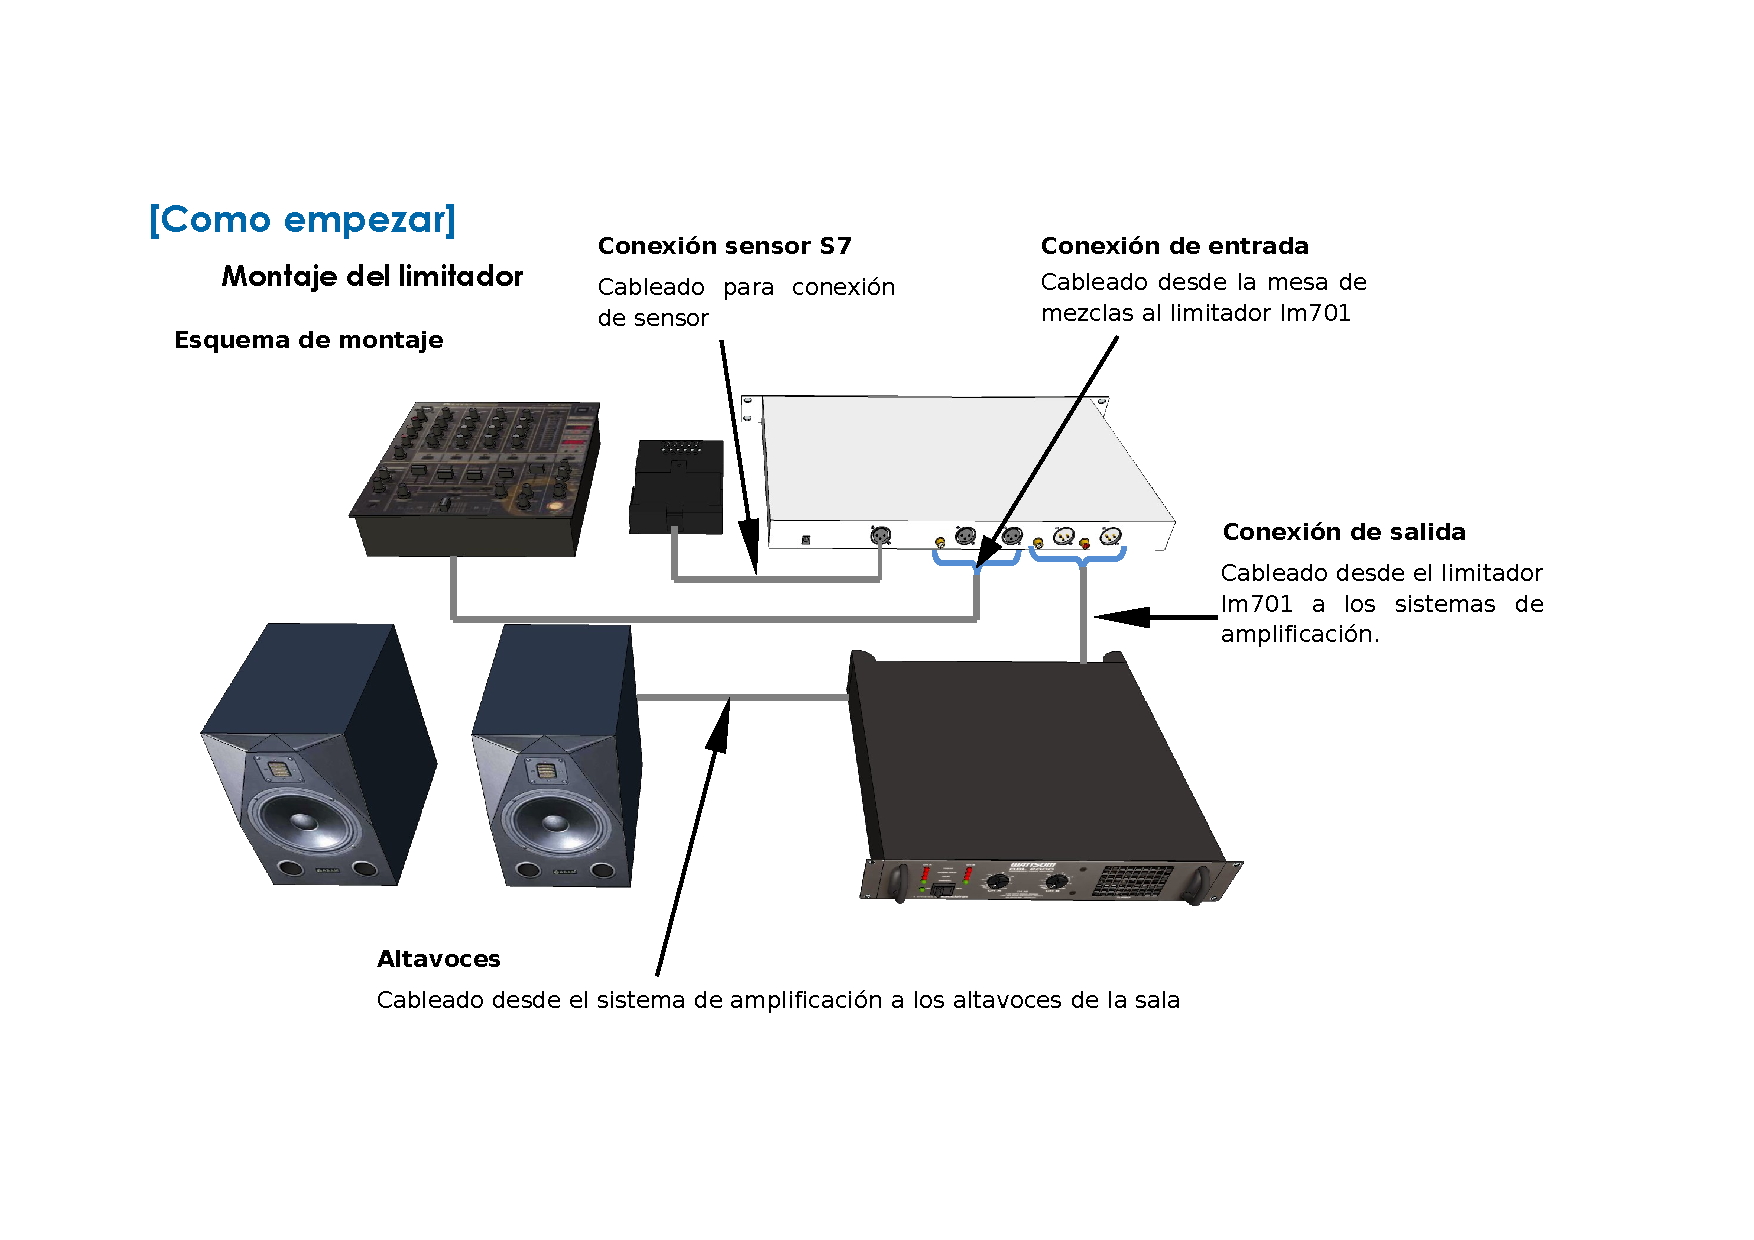
\includegraphics[scale=0.25]{figuras/manual7_montaje_trim.pdf}
%    \caption{Esquema conceptual del montaje del \acrshort{LM7}.}
%    \label{fig:lm7_montaje}
%\end{figure}

% Lo encaja en el punto actual del documento
\begin{center}
    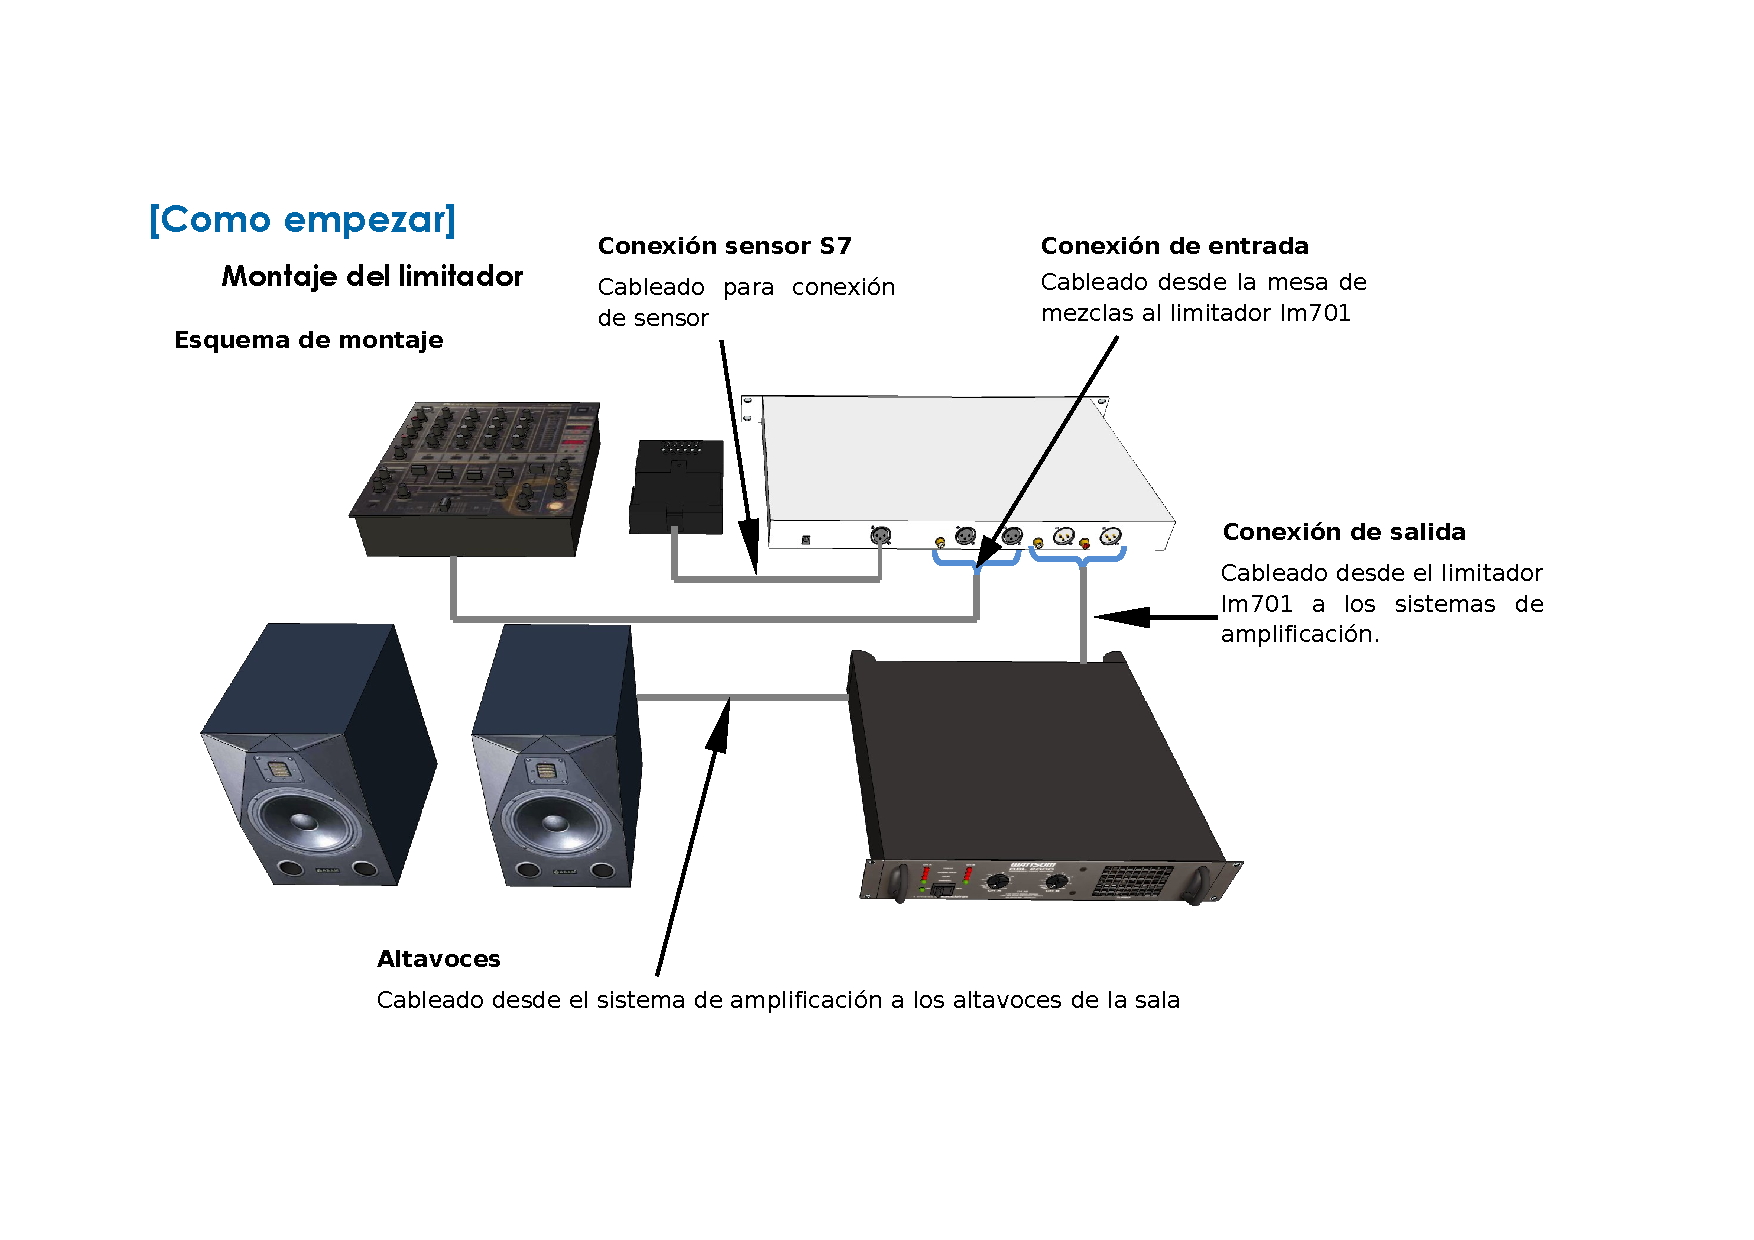
\includegraphics[scale=0.6]{figuras/manual7_montaje_trim.pdf}
    \captionof{figure}{Esquema conceptual del montaje del \acrshort{LM7}}
    \label{fig:lm7_montaje}
\end{center}

En la figura superior, podemos observar de izquierda a derecha y de arriba a bajo los siguientes elementos: mesa de mezclas (entrada), micrófono del limitador, limitador de sonido \acrshort{LM7}, altavoces, amplificador (salida).

%\begin{figure}[H]
%    \centering
%    \includegraphics[scale=0.6]{figuras/manual7_trasera_trim2.pdf}
%    \caption{Parte trasera. Conexiones del \acrshort{LM7}.}
%    \label{fig:lm7_trasera}
%\end{figure}
\begin{center}
    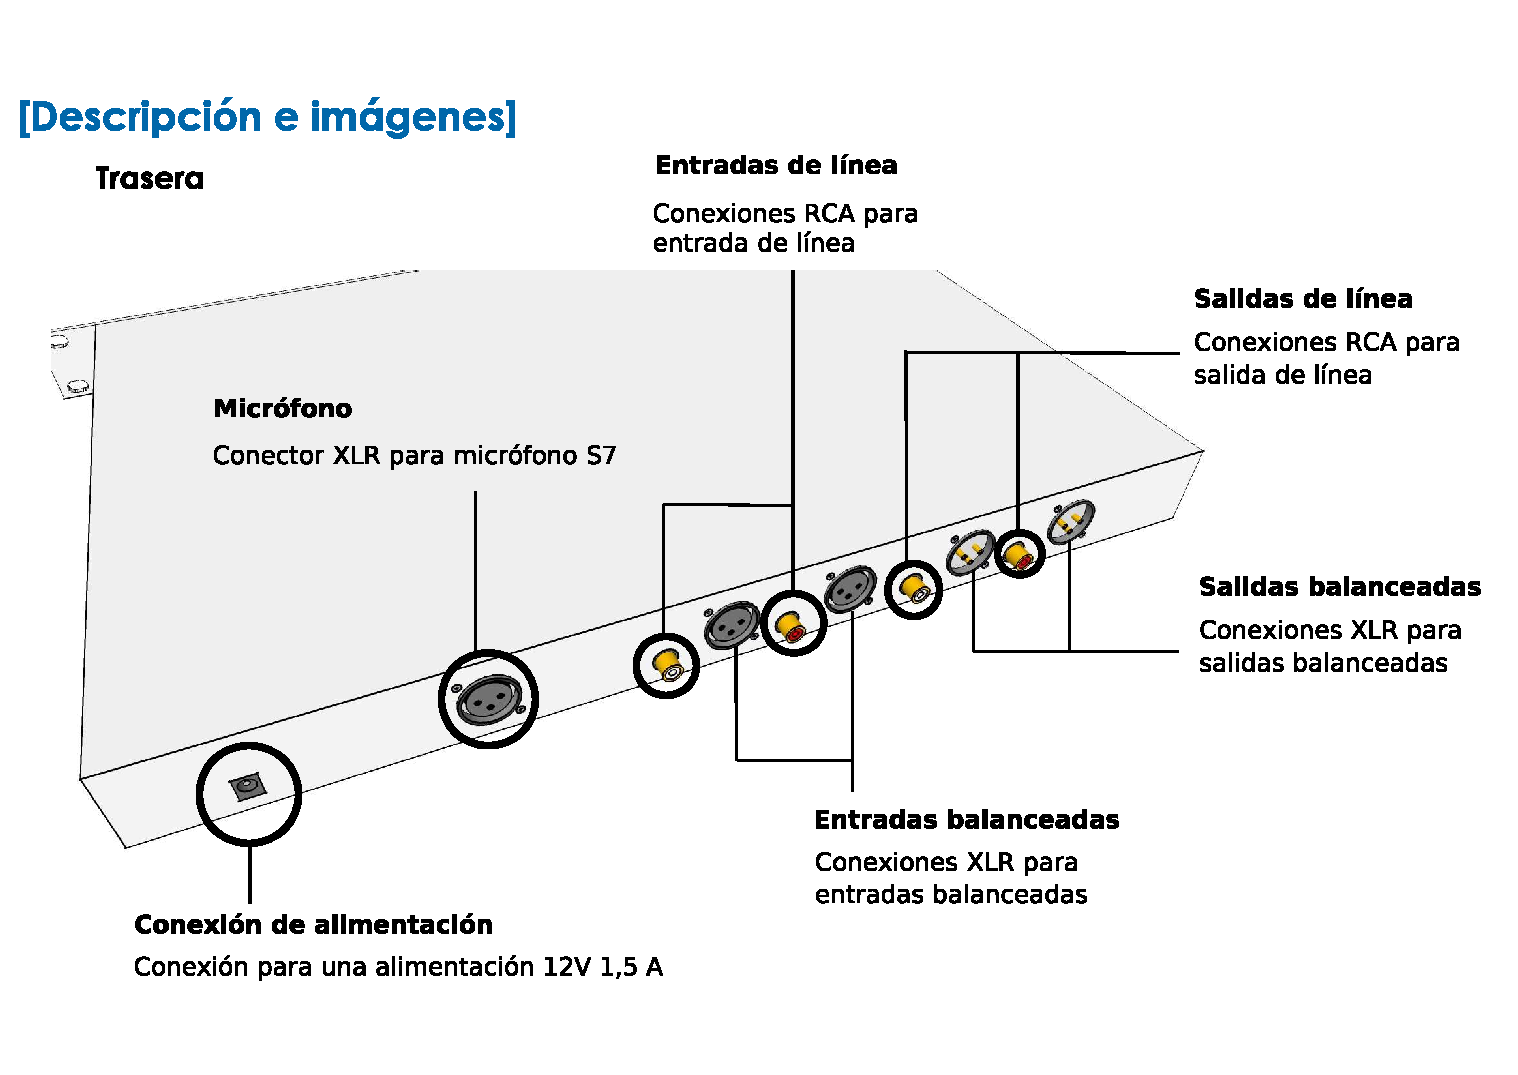
\includegraphics[scale=0.55]{figuras/manual7_trasera_trim.pdf}
    \captionof{figure}{Parte trasera. Conexiones del \acrshort{LM7}}
    \label{fig:lm7_trasera}
\end{center}

El sensor S7 (micrófono) es un componente esencial del limitador y forma parte del mismo. Gracias a él, el limitador puede medir la presión acústica en cada momento y actuar en consecuencia. Asimismo, y como se verá más adelante en este documento, será un elemento esencial en la calibración del limitador. El resto del elementos que se muestran en la figura \ref{fig:lm7_montaje} son elementos externos al limitador, y no alteran el funcionamiento del sistema en ninguna forma.

En la figura \ref{fig:lm7_trasera} se pueden observar las principales conexiones del \acrshort{LM7}, las cuales constan de:

\begin{itemize}
    \item Toma de alimentación eléctrica.
    \item Sensor S7 (micrófono) con conector \acrshort{xlr}.
    \item Entradas balanceadas para audio con conectores \acrshort{xlr}.
    \item Salidas balanceadas para audio con conectores \acrshort{xlr}.
    \item Entradas y salidas no balanceadas con conectores \gls{RCA}.
    \item Conector \glsname{rj45} para conexión directa en área local (parte frontal del limitador, no visible en las figuras).
\end{itemize}

Conectamos el micrófono al limitador, así como la entrada y la salida de audio. La salida de audio se conecta a un amplificador de sonido disponible en el laboratorio, y como salida a este sistema de amplificación se conecta un dodecaedro. De forma que podamos tener interacción con el equipo, abrimos el limitador retirando la carcasa metálica exterior, para así poder conectar un teclado y una pantalla a la placa base del equipo. De esta forma descubrimos pro primera vez las entrañas del limitador, y nos encontramos con una tecnología bastante desfasada y un ensamble prácticamente casero. Tal y como podemos ver en la imagen \ref{img:lm7}, el \gls{HW} del limitador se compone de una placa base de tipo industrial, cuyas características de detallan en la tabla \ref{tab:lms7_specs}, un circuito integrado para las entradas y salidas de audio del limitador vistas en la figura \ref{fig:lm7_trasera} y una pequeña caja negra, la cual contiene un relé, y cuya funcionalidad se verá más adelante. Además de esto podemos observar la existencia de una tarjeta de sonido \acrshort{USB} conectada a un puerto \acrshort{USB} de la placa base y cuyas salidas van hacia la caja negra que podemos ver en la imagen. Como dispositivo de almacenamiento interno tenemos un \glsname{CF}, con 1GB de capacidad. En fases posteriores del actual proceso de ingeniería inversa extraeremos esta tarjeta de almacenamiento para acceder a sus archivos, ya que será necesario descubrir o modificar las credenciales de acceso tanto al equipo como al sistema de limitación, pues todas ellas son, por ahora, desconocidas.

!! IMAGEN DEL LIMITADOR ABIERTO
\label{img:lms7_open}

Tras revisar todas las conexiones, conectamos el equipo a la corriente eléctrica, y podemos por primera vez ver el equipo en funcionamiento. Mientras arranca el sistema, vemos en la pantalla que el sistema operativo instalado es Debian, una distribución de \gls{GNU/Linux} que se caracteriza por ser minimal. Esta versión en concreto no contiene interfaz gráfica.

Una vez completado el arranque, la pantalla se llena de caracteres que desaparecen rápidamente dando lugar a otros nuevos. De entre lo que es posible leer, se deduce que estos caracteres son datos relativos al limitador (su estado en cada momento, conteniendo lecturas de micrófono y líneas, atenuación aplicada, etc) y que los procesos del limitador vuelcan sus salidas por pantalla a la salida estándar, saturando la terminal principal y dejándola inutilizable. Por tanto, se accede a otra terminal (TTY) mediante la cual podamos trabajar. Esta nueva terminal nos pide usuario y contraseña, las cuales desconocemos.

Continuando con el manual de usuario se descubre que el equipo tiene un servidor web en el cual hay desplegada una interfaz web del limitador, mediante la cual podemos ver su estado, modificar sus configuraciones y obtener informes. Por ello, el próximo y último paso para completar la instalación del limitador es conectarlo a una red interna vía Ethernet, así como conectar y configurar un ordenador adicional mediante el cual podamos acceder, no solo a dicha interfaz web, sino al equipo en sí mediante \acrshort{SSH}.

%\begin{center}
%    \hspace{0cm}
%    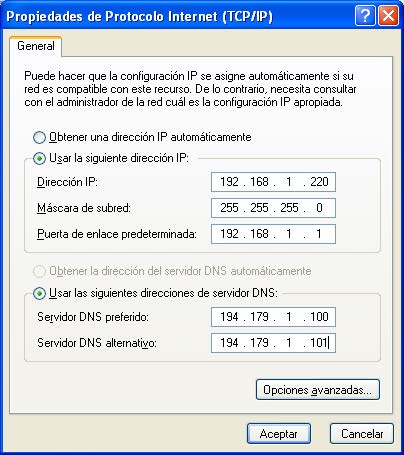
\includegraphics[scale=0.7]{imagenes/lms_ip.jpg}
%%    \captionof{figure}{Configuracion \acrshort{IP} del PC adicional}
%%    \captionof{figure}{C}
%    \hspace{2cm}
%    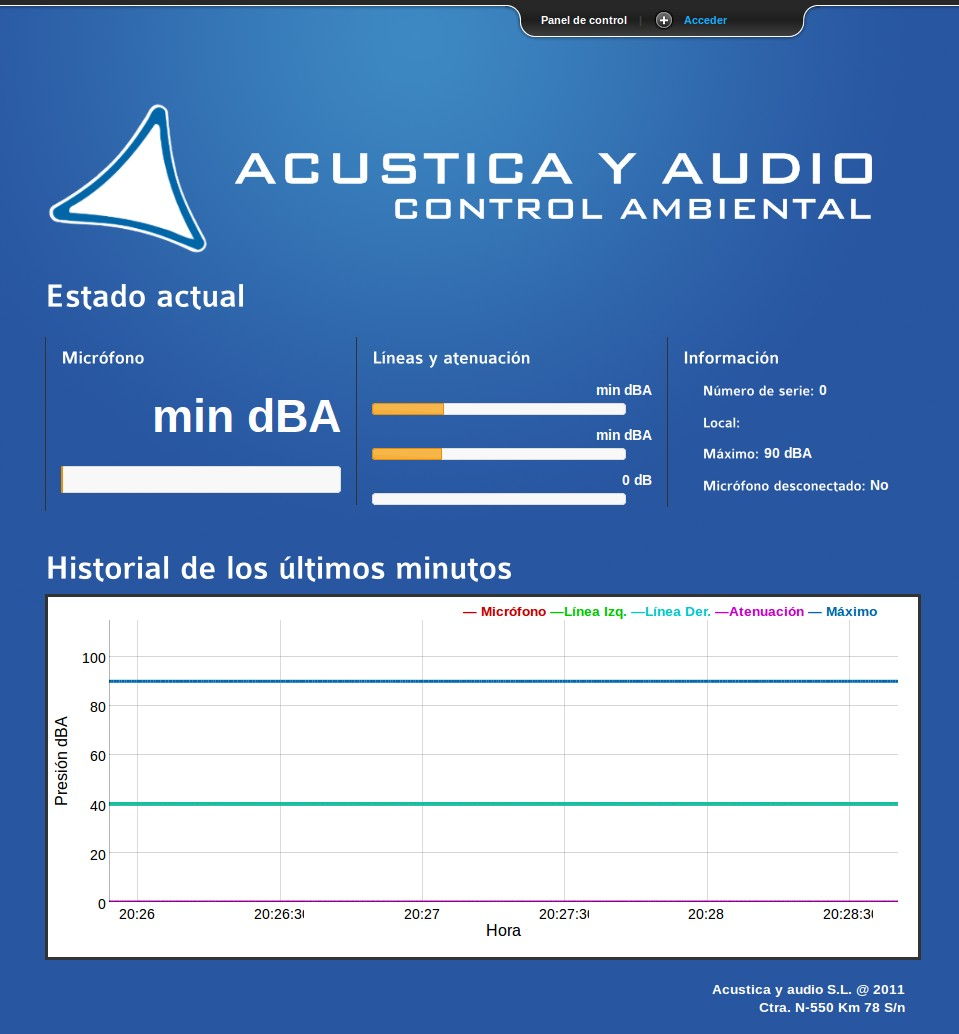
\includegraphics[scale=0.55]{imagenes/lms_ui.jpg}
%%    \captionof{figure}{Interfaz Web de \acrshort{LM7}}
%%    \caption{figure}{C}
%\end{center}

\begin{figure}[ht]
    \begin{minipage}[b]{.45\textwidth}
        \centering
        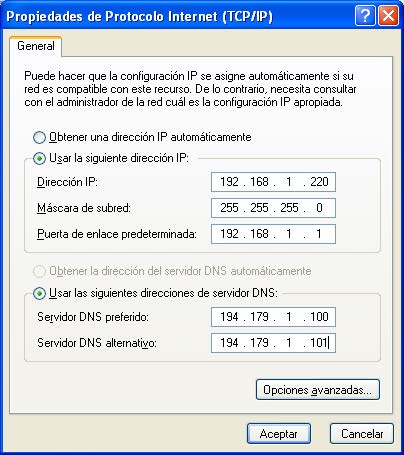
\includegraphics[width=1\textwidth]{imagenes/lms_ip.jpg}
        \caption{Configuración \acrshort{IP} requerida  en el \acrshort{PC} adicional para conectarse al limitador}
        \label{img:lms_ip}
    \end{minipage}
    \hfill
    \begin{minipage}[b]{.45\textwidth}
        \centering
        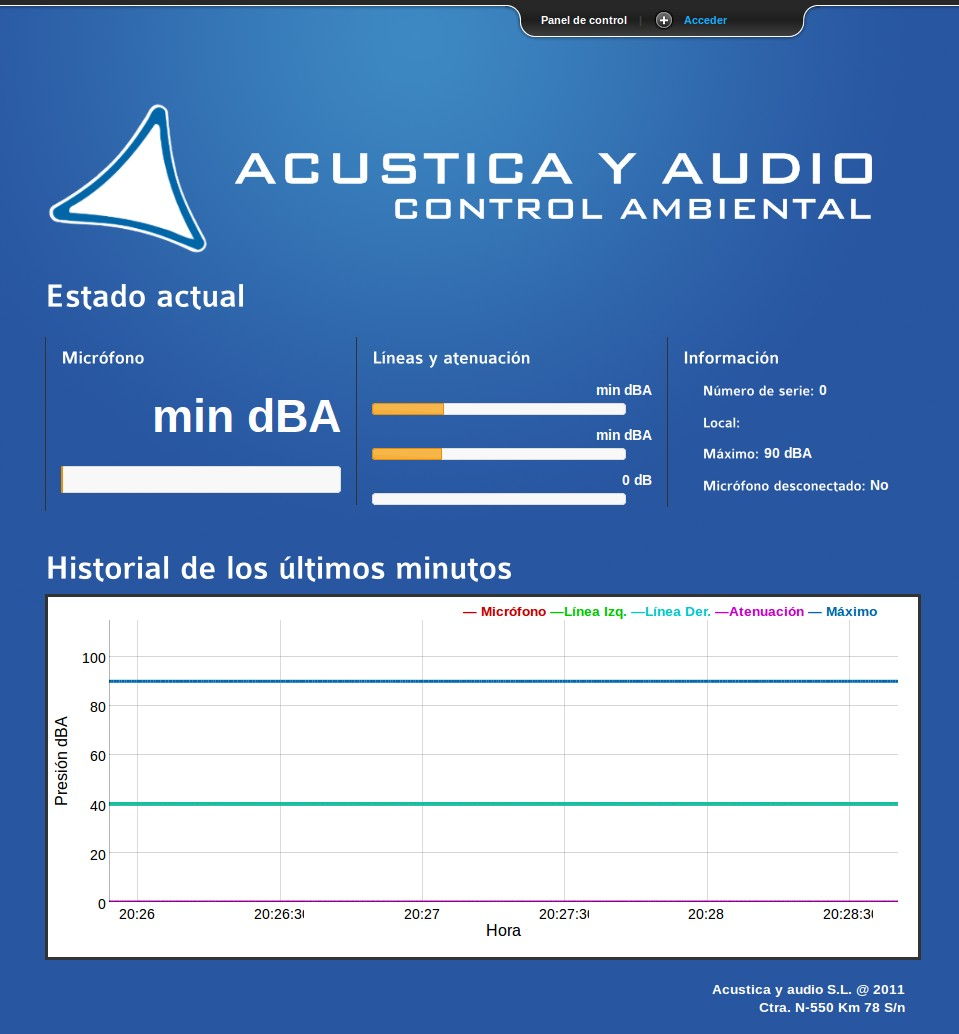
\includegraphics[width=1\textwidth]{imagenes/lms_ui.jpg}
        \caption{Interfaz web del \acrshort{LM7} \newline\newline}
        \label{img:lms_ui}
    \end{minipage}
\end{figure}

Una vez aplicada la configuración \acrshort{IP} que se muestra en la imagen \ref{img:lms_ip} en el equipo auxiliar, probamos a acceder a la interfaz web de limitador que se encuentra desplegada en la dirección \acrshort{IP}
\href{http://192.168.1.223}{http://192.168.1.223} y vemos por primera vez la aplicación web vista en la imagen \ref{img:lms_ui}. Al entrar en la interfaz web del limitador puede verse la ventana de estado, que informa sobre el estado actual del limitador. Esta interfaz arroja información básica, como:

\begin{itemize}
    \item La presión actual en \glsname{dba} tanto de las líneas como del sensor.
    \item Atenuación aplicada por el limitador en ese instante.
    \item El número de serie del limitador.
    \item El local de instalación
    \item Si el sensor (micrófono) se encuentra conectado o no.
    \item Un gráfico de los últimos 5 minutos de actuación del limitador.
\end{itemize}

En la zona superior derecha, se puede acceder al panel de control y a la sección de obtención de informes. Mediante este panel de control podremos también acceder y modificar la configuración del limitador, aunque para ellos será necesario proveer una clave de acceso válida. En el manual de usuario, se indica que existe un usuario \textit{consultor}, cuya contraseña es a su vez \textit{consultor}. Se trata de un usuario sin privilegios mediante el cual podremos consultar la configuración actual del limitador. Podemos a su vez cerrar sesión mediante el botón \commillas{Cerrar sesión}. Para poder acceder más allá necesitamos averiguar las claves de acceso al limitador.

Para acabar con el proceso de instalación, se comprueba si es posible conectarse mediante \acrshort{SSH} al limitador. Tal y como se esperaba hay conectividad entre los equipos pero necesitamos proporcionar un usuario y una contraseña para acceder al sistema operativo.

Llegados a este punto, el limitador se encuentra instalado y funcionando, pero nuestro control sobre el mismo es completamente nulo ya que no disponemos de las credenciales necesarias para acceder al sistema ni al limitador. Por tanto, procederemos a extraer su dispositivo de almacenamiento, una \glsname{CF}, para investigar desde otro ordenador su contenido y poder encontrar dichas credenciales, dando lugar así al proceso que da nombre a este capítulo, comenzaremos con el proceso de Ingeniería Inversa.

\subsection{Resumen} \label{cap1:sec1:resumen}

Como resumen a esta sección, se han realizado las siguientes acciones:

\begin{enumerate}
    \item Se ha conectado el limitador \acrshort{LM7} a corriente y se han conectado a él un monitor (interfaz VGA) y un teclado (interfaz PS/2).
    \item Se ha instalado un \acrshort{PC} auxiliar con el sistema operativo \gls{WINDOWS} 10.
    \item Se han conectado los dos equipos mediante Ethernet, usando un Switch de la marca OvisLink, con la configuración de red vista en la imagen \ref{img:lms_ip}.
\end{enumerate}

Como consecuencia de dichas acciones, tenemos los dos equipos conectados en red, por lo que se puede acceder al limitador desde el equipo auxiliar mediante \acrshort{SSH}, aunque desconoce el usuario y contraseña del sistema.

\section{Extracción de credenciales}

Para conseguir el acceso al sistema limitador, extraemos el dispositivo de almacenamiento y lo exploramos en otro ordenador mediante un adaptador. Explorando el sistema de archivos se descubre la existencia de un directorio peculiar dentro del directorio \textit{/var} en el nivel principal de la estructura de directorios de Linux.

\begin{center}
    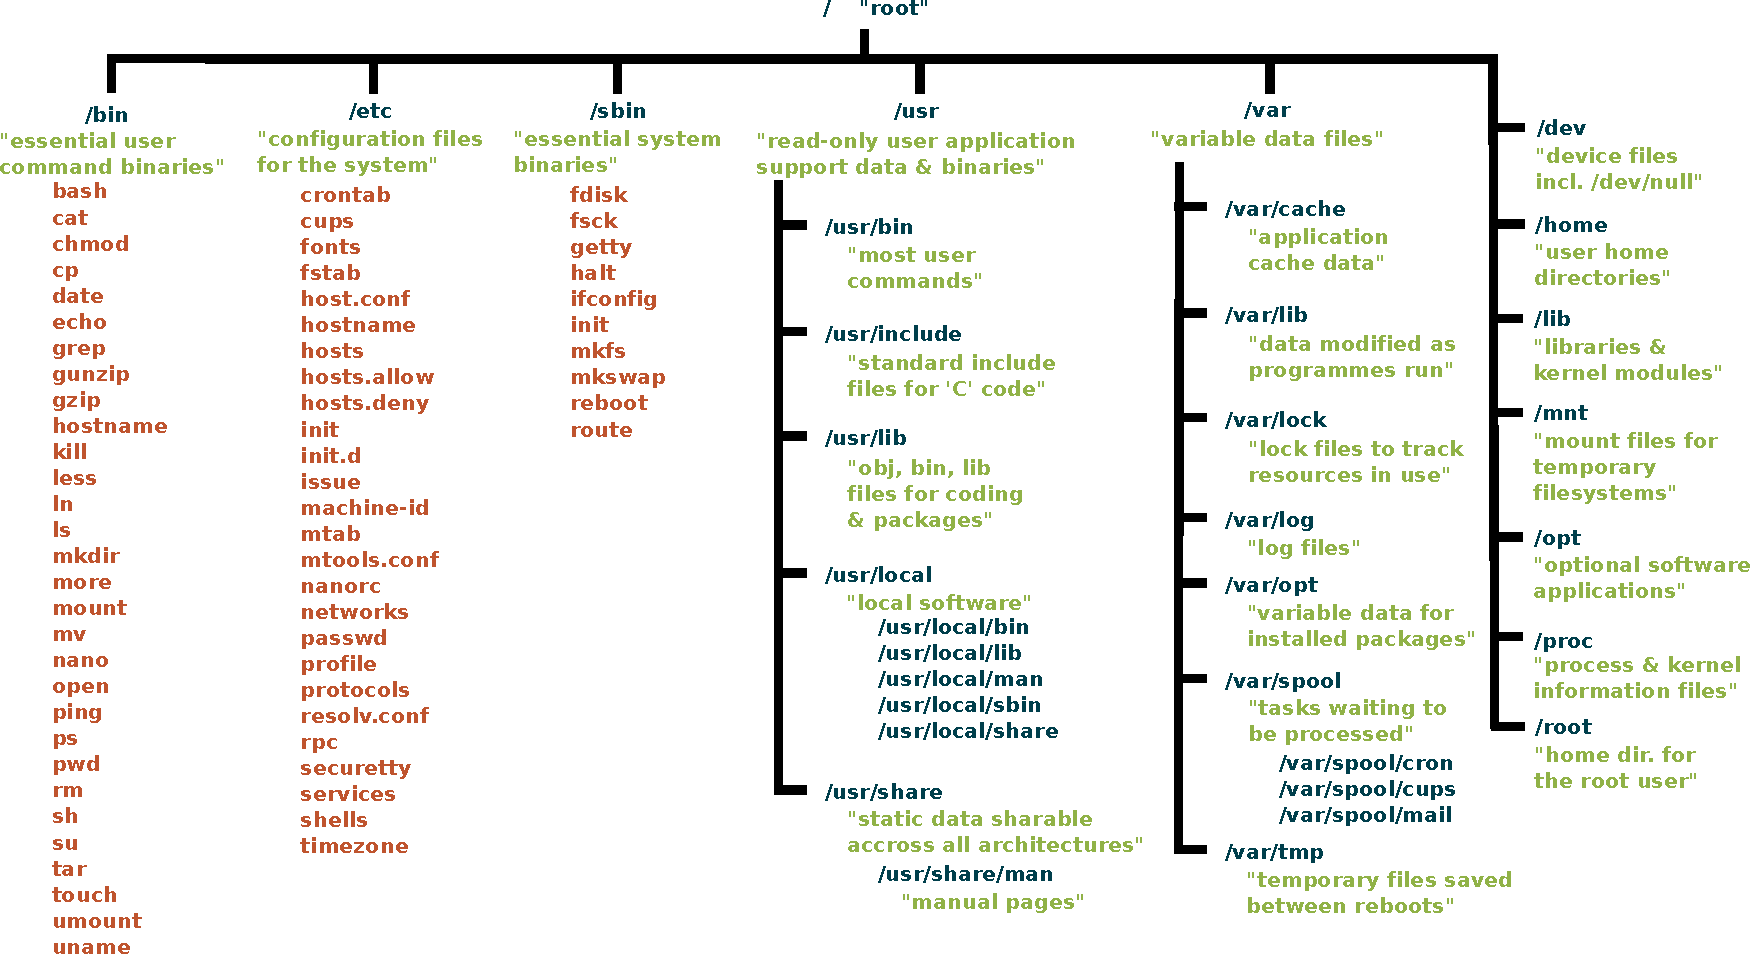
\includegraphics[scale=0.5]{figuras/unix_filesystem_hierarchy.pdf}
    \captionof{figure}
    {
        Estructura de directorios de un sistema \gls{GNU/Linux} \\
        Fuente : \cite{wikipedia}
%        Fuente: \href{https://upload.wikimedia.org/wikipedia/commons/f/f3/Standard-unix-filesystem-hierarchy.svg}{Wikipedia}
    }
    \label{fig:dirs_linux}
\end{center}

\subsection{Credenciales del limitador}

Dentro de esta carpeta denominada \textit{slr/} encontramos rápidamente un fichero llamado \textbf{\textit{users.auth}}, con usuarios, claves y permisos. Estas credenciales no son las del sistema operativo que corre sobre la máquina, sino las de los usuarios que tienen acceso a la configuración del limitador, es decir, son los usuarios y contraseñas necesarios para acceder a la aplicación web del limitador (imagen \ref{img:lms_ui}), así como los permisos de estos usuarios sobre la configuración del limitador.

\begin{shaded}
%    \textbf{\textit{slr/}}
    \noindent
    El directorio \textbf{slr/} será de gran importancia en el ámbito del proyecto, ya que en este directorio se almacenarán la gran mayoría de ficheros relacionados con el limitador: datos de configuración, información de usuarios, ficheros de sonido, e incluso ficheros que funcionarán a modo de variables globales del limitador. Conforme se vaya avanzado en el documento se irá describiendo y explicando cada uno de estos ficheros.
    \par
    \noindent
    El nombre del directorio se deduce que es un acrónimo de \textit{\textbf{S}ound\textbf{L}imiter\textbf{R}ecords}.
\end{shaded}

Para nuestra sorpresa, se descubre que los datos no sólo están almacenados en un fichero de texto plano, sino que tampoco se encuentran cifrados. Cada una de las líneas del fichero define un usuario con los siguientes campos:

\begin{itemize}
    \item \acrshort{dni}.
    \item Nombre.
    \item Contraseña.
    \item Gestor de usuarios (si puede crear, modificar o eliminar usuarios).
    \item Gestor de configuración (si puede modificar la configuración del limitador).
    \item Fecha del alta del usuario en el sistema.
\end{itemize}

En el listado \ref{lst:usersAuth} pueden verse claros ejemplos del patrón definido justo sobre estas líneas. Adicionalmente, existen en el fichero otras líneas que no siguen este patrón y definen otros patrones nuevos. Ejemplos de estas líneas son las que encontramos en la línea 4 y 14 del listado \ref{lst:usersAuth}. Estas líneas definen el modo de acceso al limitador y la eliminación de un usuario en el sistema, respectivamente, así como la marca de tiempo de la acción que dio origen a la inserción de esas líneas en el fichero.

Para confirmar el descubrimiento de las credenciales del limitador se comprueban algunos de los usuarios y claves encontradas en la interfaz web del limitador, con resultado satisfactorio. Se consigue por tanto el acceso a la configuración del limitador y tenemos ahora el control sobre él, aunque seguimos sin disponer de control sobre el sistema operativo sobre el que corre.\newline

\begin{lstlisting} [language=HTML, label={lst:usersAuth}, caption={Contenido del fichero \textit{users.auth}}]
    dni=*lm7-passwordUser&name=Password user&password=\t****&userManager=1&configManager=1&time=2012/05/11-11:48:36
    dni=*lm7-remoteUser&name=Remote system user&password=\t****&userManager=0&configManager=0&time=2012/05/11-11:48:36
    dni=consultor&name=Consultor&password=consultor&userManager=0&configManager=0&time=2012/05/11-11:48:36
    key=authMethod&value=onlyPassword&time=2012/08/30-05:35:16
    dni=E19578186&name=NOISEOFF&password=COCHA012015&userManager=1&configManager=1&time=2015/06/25-23:07:38
    dni=E19578186&name=NOISEOFF&password=COCHA012015&userManager=1&configManager=1&time=2015/06/25-23:08:13
    dni=E19578186&name=NOISEOFF&password=01COCHA2015&userManager=1&configManager=1&time=2015/06/26-14:55:51
    key=authMethod&value=onlyPassword&time=2015/06/26-14:57:58
    dni=E19578186&name=NOISEOFF&password=COCHA0130115&userManager=1&configManager=1&time=2016/09/20-19:14:48
    dni=E19578186&name=NOISEOFF&password=COCHA0130115&userManager=1&configManager=1&time=2016/09/20-19:16:21
    key=authMethod&value=onlyPassword&time=2016/09/20-19:16:50
    dni=E19578186&name=NOISEOFF&password=cocha0130115&userManager=1&configManager=1&time=2017/01/02-12:08:33
    dni=44289989Q&name=NOISEOFF&password=cocha0130115&userManager=1&configManager=1&time=2017/01/02-12:10:05
    dni=E19578186&deleted=1
    key=authMethod&value=onlyPassword&time=2017/01/02-12:12:01
    dni=44289989Q&name=NOISEOFF&password=cocha0130115&userManager=1&configManager=1&time=2017/01/05-09:50:40
    key=authMethod&value=onlyPassword&time=2017/01/05-09:52:03
\end{lstlisting}

\subsection{Credenciales del sistema operativo}

Para obtener el control sobre el sistema operativo es necesario disponer de un usuario y contraseña válidos de forma que podamos acceder a él mientras el equipo está en funcionamiento.

Del sistema operativo sabemos que es \gls{debian}, una distribución \gls{GNU/Linux}, por tanto, se investiga dónde almacena este sistema sus usuarios. Son datos estáticos así que deben encontrase almacenados en alguna parte dentro del sistema de archivos contenidos en el disco, el cual, recordamos, tenemos conectado a otro ordenador mediante un adaptador \acrshort{USB}.

A través de la consulta de foros
 \href{https://www.cyberciti.biz/faq/where-are-the-passwords-of-the-users-located-in-linux/}{(cyberciti.biz)} y manuales \href{https://www.debian.org/doc/manuals/system-administrator/ch-sysadmin-users.html}{(Debian.org)} en línea, descubrimos que los ficheros que necesitamos son \textbf{/etc/passwd} y \textbf{/etc/shadow}. Aunque ambos contienen información crítica sobre los usuarios y sus permisos, existen pequeñas diferencias. En resumen, mientras que \textbf{/etc/passwd} almacena información mayormente relativa al usuario, \textbf{/etc/shadow} contiene las claves de usuario (encriptadas) e información relacionada a ellas, no al usuario.

%El fichero \textbf{/etc/shadow} contiene una entrada por línea para cada uno de los usuarios listados en el fichero \textbf{/etc/passwd}. Las claves están compuestas por una serie de campos, separados por dos puntos (:), y son de la siguiente manera:

Las contraseñas encriptadas y otra información relacionada, como la información de caducidad de la contraseña, se almacenan en el fichero \textbf{/etc/shadow}. Este fichero contiene una entrada por línea por cada uno de los usuarios listados en el fichero \textbf{/etc/passwd}. Cada una de estas entradas están compuestas por una serie de campos separados por dos puntos (:), y generalmente, sigue este patrón.

\begin{center}
    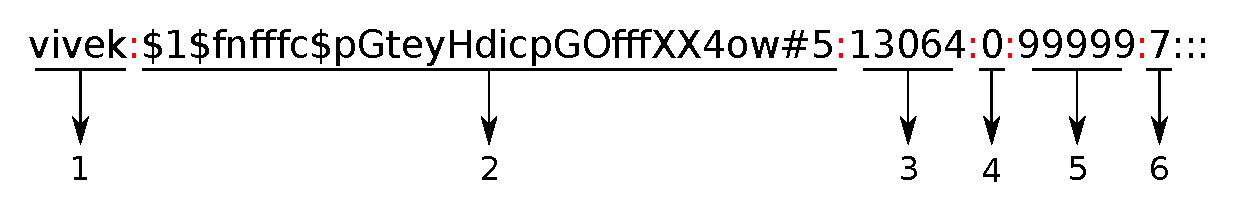
\includegraphics[scale=0.5]{figuras/shadow.pdf}
    \captionof{figure}{Estructura de las claves en el fichero \textbf{/etc/shadow}}
    \label{fig:shadow}
\end{center}

\begin{enumerate}
    \item Nombre de usuario.
    \item Contraseña encriptada (\textbf{hash}). Sigue el formato \textbf{\textdollar id\textdollar salt\textdollar hash}. El campo \textbf{\textdollar id} representa el algoritmo usado:
        \begin{enumerate}
           \item \textbf{\textdollar 1\textdollar } es MD5.
           \item \textbf{\textdollar 2a\textdollar} es Blowfish.
           \item \textbf{\textdollar 2y\textdollar} es Blowfish.
           \item \textbf{\textdollar 5\textdollar } es SHA-256.
           \item \textbf{\textdollar 6\textdollar } es SHA-512.
        \end{enumerate}
    \item Días desde que se cambió la contraseña, contando desde el 1 de enero de 1970.
    \item Días tras los cuales la contraseña debe ser cambiada.
    \item Días de antelación a la expiración de la contraseña en los que se avisa al usuario.
    \item Días tras los cuales se desactiva una cuenta cuya contraseña está caducada.
\end{enumerate}

\begin{shaded}
    \noindent
    Una contraseña \textbf{hash} no es más que una cadena de caracteres única, la cual es resultado de la ejecución de un algoritmo de encriptación, dada otra cadena de caracteres como entrada. Esta contraseña \textbf{hash} es la que se almacena en el sistema, y no la contraseña original. Durante el proceso de inicio de sesión, se comprueba el \textbf{hash} de la contraseña insertada por el usuario y la contraseña \textbf{hash} almacenada, verificando así la integridad de la misma.
\end{shaded}

Abrimos el fichero \textbf{/etc/shadow} y encontramos la información que necesitamos. La imagen \ref{img:shadow} muestra el contenido de este fichero.

\begin{center}
    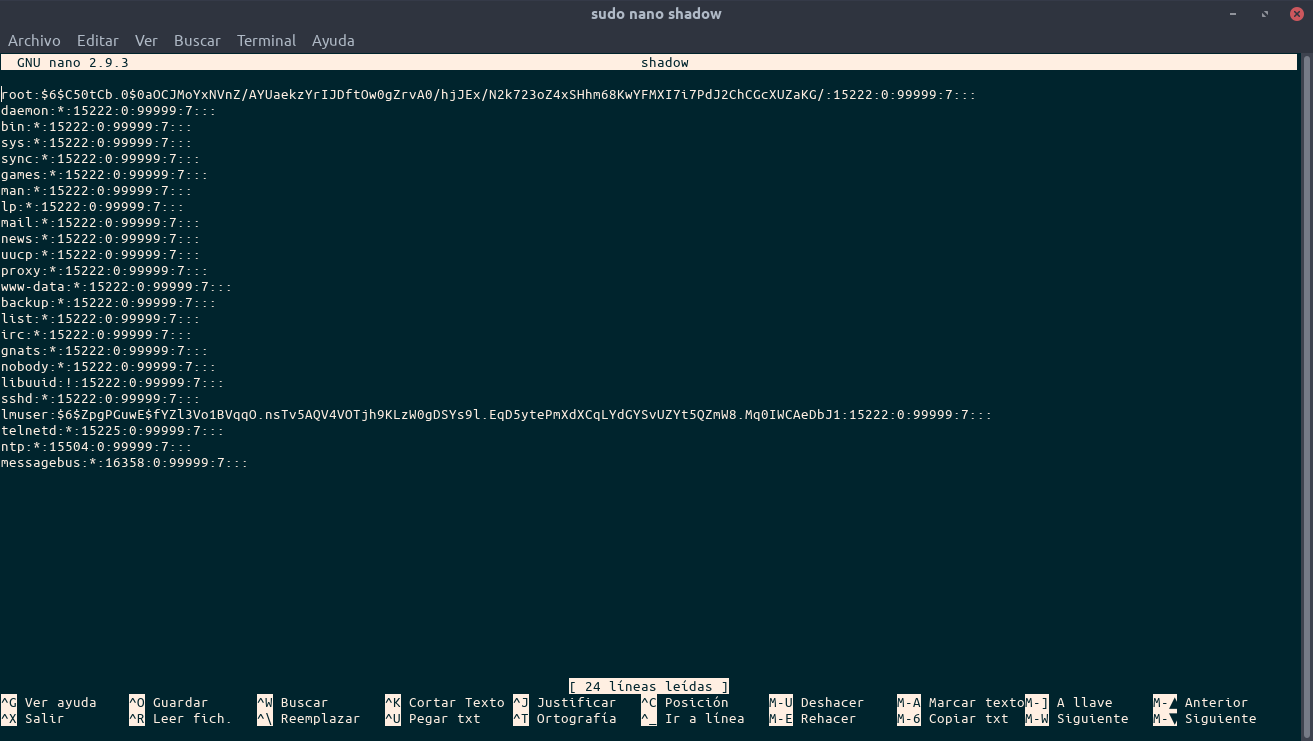
\includegraphics[scale=0.25]{imagenes/shadow.png}
    \captionof{figure}{Contenido del fichero \textbf{/etc/shadow} del \gls{LM7}}
    \label{img:shadow}
\end{center}

Los usuarios que nos interesan son \textbf{root} y \textbf{lmuser}. Ambas contraseñas se han cifrado usando el algoritmo SHA-512, ya que su primer campo es \textdollar 6\textdollar. En un primer intento se modifica el fichero y se eliminan los campos que contienen la contraseña \textit{Hash}, con la intención de forzar el inicio de sesión sin la necesidad de contraseña (contraseña vacía). Sin embargo, este enfoque no produce el resultado esperado y se busca otra solución. \\ Como conocemos tanto el formato de las entradas de este fichero como el algoritmo de cifrado utilizado, el segundo enfoque será sustituir estas claves \textit{Hash} con otras nuevas, generadas por nosotros. Generamos una nueva contraseña usando la utilidad \gls{openssl}.\newline

\begin{lstlisting}[language=bash, label={lst:openssl}, caption={Generación de Hash usando cifrado SHA-512}]
    $~ openssl passwd -6 <cadena>
\end{lstlisting}

La ejecución del comando \ref{lst:openssl} nos genera una clave Hash única para la cadena que le proporcionemos como entrada. La opción -6 indica que debe usarse el algoritmo de cifrado SHA-512. Para más información sobre este comando y sus opciones puede consultarse la documentación oficial \cite{openssl}.

Una vez cambiadas las contraseñas por las que hemos generado, re-instalamos el \glsname{CF} en la placa base del limitador y se procede a encenderlo para comprobar que podemos acceder al sistema con las nuevas credenciales. Tras finalizar el arranque se verifica que el inicio de sesión con ambos usuarios es satisfactorio, y que por tanto, se tiene control sobre el sistema operativo. La conexión al equipo mediante \acrshort{SSH} también funciona correctamente usando las nuevas contraseñas. Anteriormente, se ha comprobado que la configuración \acrshort{SSH} del sistema permite la conexión mediante el usuario \textit{root}. Para ello se comprueba que en el fichero de configuración en la ruta /etc/sshd\textunderscore conf contiene la directiva \textit{PermitRootLogin} y que su valor es YES. Tras comprobar el fichero, se verifica que la directiva existe y está configurada correctamente. Este no es el valor por defecto, por lo tanto ha tenido que ser activado con anterioridad. Además, se añade la siguiente directiva para garantizar el acceso a los usuario \textit{root} y \textit{lmuser}: \newline

\begin{lstlisting}[nolol, language=XML, label={lst:confSSH}, caption={Directiva del fichero}]
    AllowUsers root lmuser
\end{lstlisting}

\section{Especificaciones del sistema}

El primer paso para comenzar a investigar el equipo es descubrir ante que tipo de hardware nos enfrentamos. En secciones anteriores (imagen \ref{img:lms7_open}) se mostró el hardware del limitador bajo estudio, y se comentó brevemente sus características. En esta sección, se va a realizar un análisis más profundo sobre las capacidades y características hardware del sistema:

Nos encontramos antes un equipo en el que se ha montado una placa base de tipo industrial, en la que vienen integrados todos los recursos hardware necesarios para correr un sistema operativo. En la siguiente tabla pueden verse los componentes básicos con los que cuenta el sistema:

%\begin{itemize}
%    \item Placa base: ALIX-1E
%    \item CPU: AMD Geode LX
%        \begin{itemize}
%            \item Núcleos: 1
%            \item Velocidad: 433/500MHz
%        \end{itemize}
%    \item Memoria: 128/256MB SDRAM
%    \item Almacenamiento: CompactFlash 1GB
%    \item Audio: AMD CS5536 chip \cite{cs5536}
%    \item Interfaces:
%        \begin{itemize}
%            \item x2\glsname{COM}
%            \item x4\glsname{USB}
%            \item x1\glsname{LPT}
%            \item x1\glsname{VGA}
%        \end{itemize}
%    \item Conectividad: Ethernet
%    \item Dimensiones: 17x17cm
%    \label{tab:lms7_specs}
%\end{itemize}

\begin{table}[h]
    \centering
    \begin{tabular}{|>{\columncolor[HTML]{ECF4FF}}l |l|}
        \hline
        Placa base     & ALIX-1E                    \\ \hline
        Procesador     & AMD Geode LX               \\ \hline
        Memoria        & 128/256MB SDRAM            \\ \hline
        Almacenamiento & CompactFlash 1GB           \\ \hline
        Interfaces     & 4x\glsname{USB}, 1x\glsname{VGA}, 1x\glsname{LPT}, 2x\glsname{COM} \\ \hline
        Conectividad   & Ethernet                   \\ \hline
        Dimensiones    & 17x17cm                    \\ \hline
    \end{tabular}
    \caption{Especificaciones hardware del \gls{LM7}}
    \label{tab:lms7_specs}
\end{table}

Como componentes que no forman parte de la placa base, tenemos una tarjeta de sonido USB conectada a uno de los puertos y un circuito integrado para las entradas y salidas de audio, conectado a la placa base mediante su puerto serie.

\begin{center}
    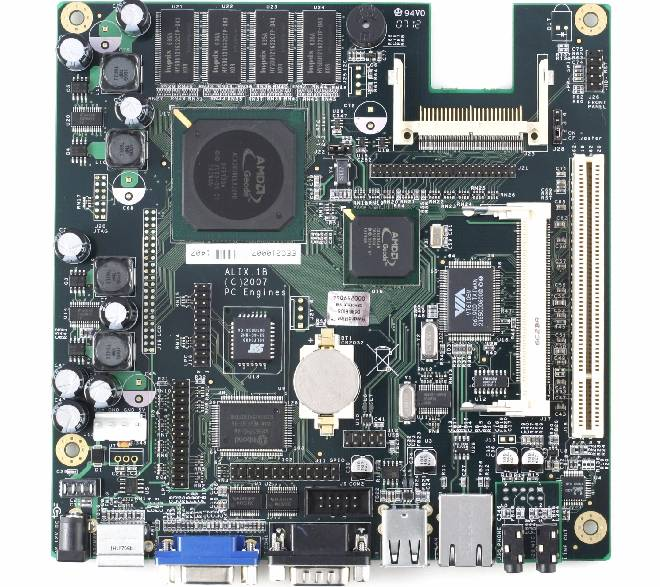
\includegraphics[scale=0.5]{imagenes/alix1b.jpg}
    \captionof{figure}{Imagen de una placa base ALIX-1B \cite{alix}}
    \label{img:alix1b}
\end{center}

\section{Análisis del rendimiento}

Tal y como se comentó en la primera sección de este capítulo, el ordenador auxiliar que se ha instalado en el laboratorio, y en red como el \gls{LM7}, tiene \gls{WINDOWS} 10 como sistema operativo. Para facilitar el acceso remoto mediante \acrshort{SSH} al equipo limitador, se hace uso de clientes \acrshort{SSH}. En la tabla \ref{tab:gestoresSSH} se lista el cliente usado tanto en Windows 10 como en Linux.

% Please add the following required packages to your document preamble:
% \usepackage{graphicx}
\begin{table}[h]
    \centering
    \begin{tabular}{|l|l|}
        \hline
        \rowcolor[HTML]{ECF4FF}
        Sistema Operativo & Cliente SSH   \\ \hline
        Linux             & Snowflake SSH \\ \hline
        Windows           & MobaXterm     \\ \hline
    \end{tabular}
    \caption{Clientes \acrshort{SSH} utilizados en el proyecto.}
    \label{tab:gestoresSSH}
\end{table}

Estos clientes aportan ciertas ventajas, como por ejemplo:

\begin{itemize}
    \item Permiten guardar los datos de acceso a equipos remotos. Una conexión \acrshort{SSH} a otro equipo se resume en hacer click sobre un botón.
    \item Proporcionan una interfaz gráfica.
    \item Disponen de un navegador de archivos.
    \item Monitorizan el sistema remoto, lo que nos permite analizar el uso de recursos (disco, memoria, \acrshort{CPU} y red) en tiempo real.
\end{itemize}

Tras configurar el cliente \acrshort{SSH}, se lanza una conexión remota al \gls{LM7}. Los datos de monitoreo muestran una alta tasa de utilización del \acrshort{CPU}, en torno al 85-100\% (ver imágenes \ref{img:lms_ps1} y \ref{img:lms_ps2}). Indudablemente, el hecho de que el \acrshort{CPU} disponga de una único núcleo es significativo, sin embargo, se procede a identificar los procesos en funcionamiento que pertenecen al limitador. Para ello, se recurre al código fuente del limitador, en concreto al fichero \gls{makefile}, el cual se encarga de compilar los distintos ejecutables (a los que llamaremos \textbf{módulos}) y de moverlos al directorio raíz del sistema: \textbf{/bin}. Al colocar los programas en esta carpeta, se pueden lanzar de forma global, es decir, sin especificar su ruta.

\begin{figure}[ht]
    \begin{minipage}[b]{.45\textwidth}
        \centering
        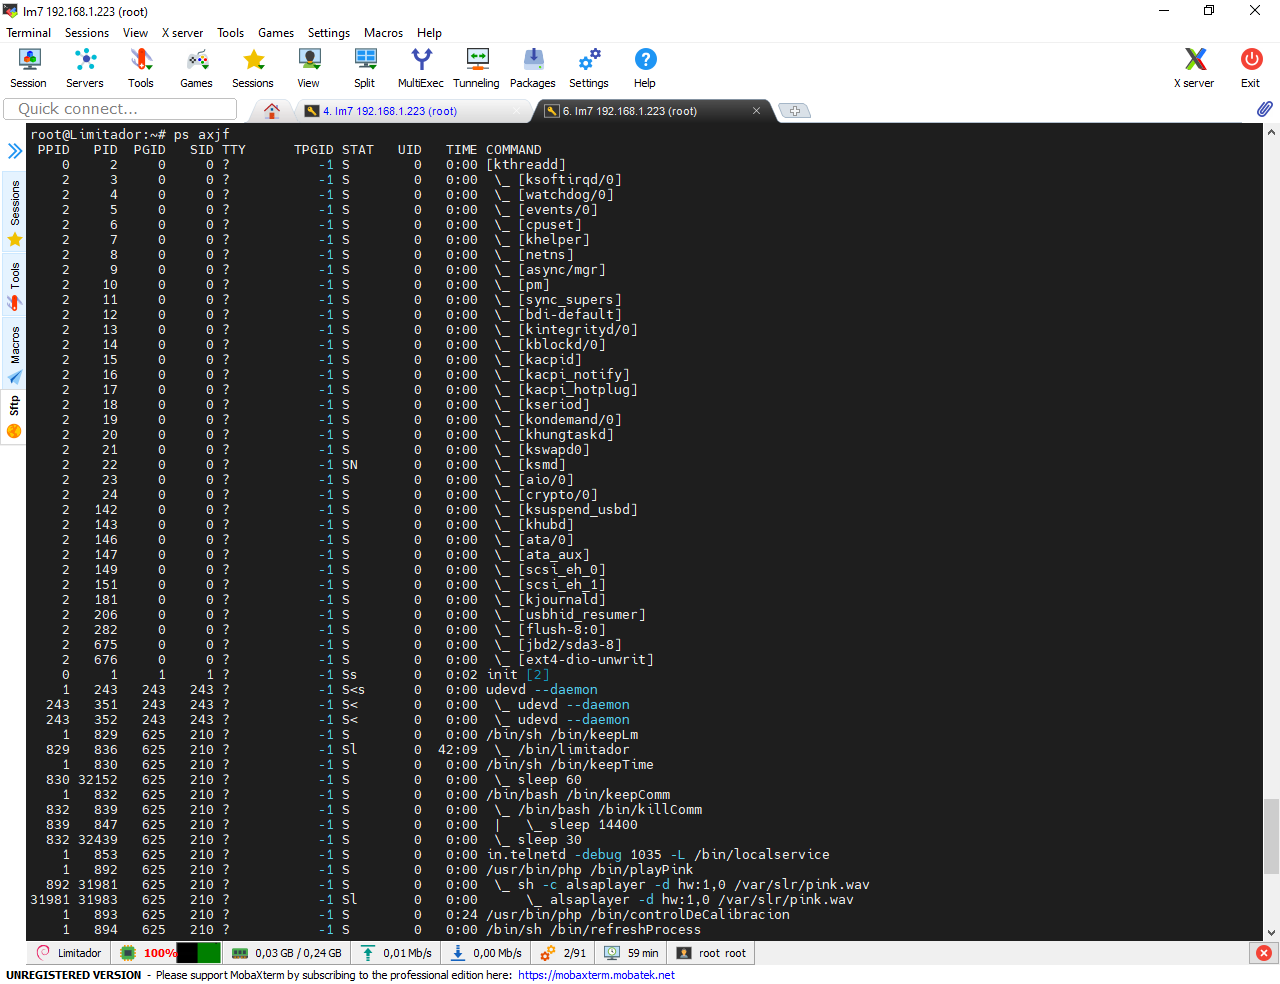
\includegraphics[width=1\textwidth]{imagenes/lm7_ps[1].png}
        \caption{}
        \label{img:lms_ps1}
    \end{minipage}
    \hfill
    \begin{minipage}[b]{.45\textwidth}
        \centering
        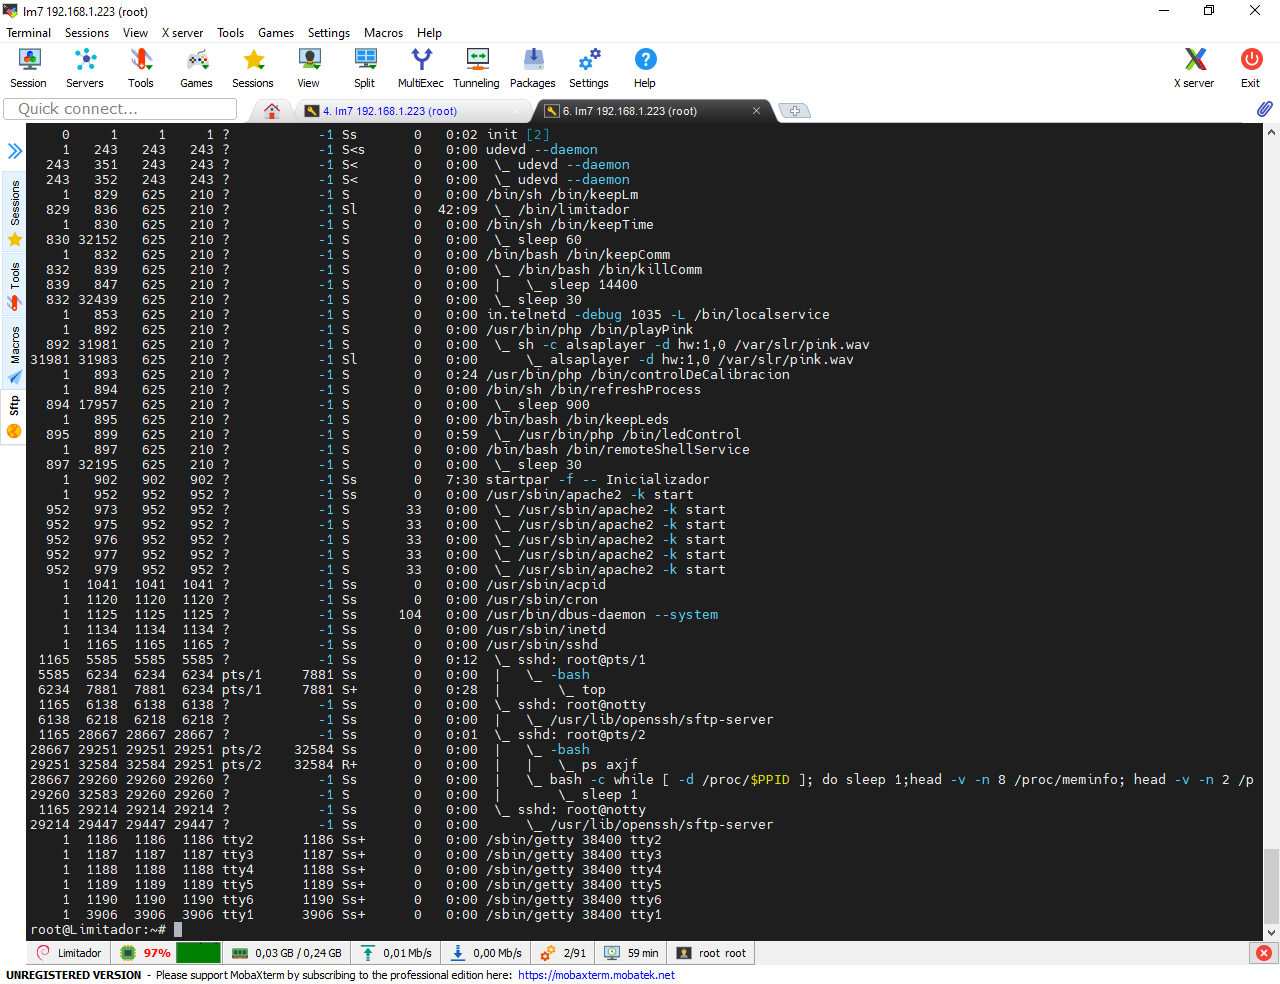
\includegraphics[width=1\textwidth]{imagenes/lm7_ps[2].png}
        \caption{}
        \label{img:lms_ps2}
    \end{minipage}
\end{figure}

El fichero \gls{makefile} nos proporciona una lista de nombres de procesos a buscar. Listamos los procesos activos con la orden \textbf{ps}. El comando completo así como el resultado devuelto pueden observarse en las captura de pantalla \ref{img:lms_ps1} y \ref{img:lms_ps2}. Las opciones pasadas al invocar al comando \textbf{ps} permite mostrar no solo los procesos en activo, sino también las relaciones jerárquicas que existen entre ellos. La mayoría de los procesos del limitador son fácilmente detectables incluso en el supuesto de que se conocieran sus nombres con anterioridad. Los procesos relativos al limitador se encuentran remarcados en rojo, y se puede apreciar el detalle de que todos ellos tiene como proceso padre  a \textbf{init}, con \acrshort{PID} 1. Podemos ver esta información en la primera columna de la tabla, \acrshort{PPID}. Esto significa que los procesos del limitador son lanzados automáticamente al arrancar el sistema.

\begin{shaded}
    \noindent
    El proceso \textbf{init} o \textbf{systemd} es un gestor de servicios para sistemas operativos Linux. Es el primer proceso en arrancar (con \acrshort{PID} 1) y el último en acabar durante el apagado. Su función es levantar los procesos a nivel de usuario.
\end{shaded}

!! EXPLICAR INIT.D

Los procesos que componen en limitador se verán con profundidad en la sección \ref{sec:lm7_procesos}, pero antes, se presentará y estudiará la interfaz web del limitador en su totalidad (ya se presentó la sección principal con la imagen \ref{img:lms_ui}), mediante la que podemos configurarlo y visualizar las lecturas de los sensores y la atenuación aplicada en cada momento.

\section{Interfaz web}

La interfaz web del limitador se encuentra desplegada en un servidor \gls{apache}, y está programada usando PHP, \acrshort{CSS}, HTML y Javascript. En la tabla \ref{tab:lm7_lamp_specs} puede consultarse un análisis más detallado de las tecnologías usadas en la interfaz web.

% Please add the following required packages to your document preamble:
% \usepackage[table,xcdraw]{xcolor}
% If you use beamer only pass "xcolor=table" option, i.e. \documentclass[xcolor=table]{beamer}
\begin{table}[h]
    \centering
    \begin{tabular}{|l|l|}
        \hline
        \rowcolor[HTML]{ECF4FF}
        \multicolumn{1}{|c|}{\cellcolor[HTML]{ECF4FF}\textbf{Tecnología}} & \multicolumn{1}{c|}{\cellcolor[HTML]{ECF4FF}\textbf{Versión}} \\ \hline
        Sistema Operativo                                                 & Debian 4.3.5                                                  \\ \hline
        Servidor Web                                                      & Apache 2.2.16                                                 \\ \hline
        PHP                                                               & 5.5.3                                                         \\ \hline
    \end{tabular}
    \caption{Especificaciones del servidor web del \gls{LM7}}
    \label{tab:lm7_lamp_specs}
\end{table}


El estudio del la interfaz representa un aspecto clave en el proceso de ingeniería inversa en el que nos encontramos. La interfaz web arroja una gran cantidad de información mediante la cual somos capaces no sólo de comprender qué hace el sistema, qué datos almacena y como los representa y exporta, sino que también nos permite generar un conjunto de requisitos funcionales, no funcionales y de datos que nuestro proyecto deberá satisfacer, y como mínimo, debe hacerlo tan bien (o mal) como el sistema estudiado (requisitos de calidad). Por otra parte, será una guía y un recurso al cual recurriremos una y otra vez a lo largo de este proyecto. En definitiva, la interfaz web nos permite, de un vistazo, comprender el sistema y sus capacidades.

\subsection{Imágenes}

En esta subsección se va a presentar las interfaz web en imágenes de forma que el lector pueda ver la interfaz web por sí mismo, aunque de forma estática. Algunas de las imágenes han sido extraídas del manual de usuario original del limitador, mientras que otras han sido directamente tomadas de la interfaz web del limitador durante su funcionamiento.

!!! meter y explicar imágenes de la interfaz

\subsection{Análisis técnico}

En esta subsección profundizamos un poco más en la interfaz web recurriendo a su código fuente. Bajamos por tanto un escalón importante a nivel de abstracción. Por razones obvias, no se va a incluir la totalidad del código de la interfaz web del limitador en esta subsección, sino que se va a realizar un análisis técnico del mismo, destacando las cualidades o deficiencias más importantes que se han detectado y presentando bloques de código que den soporte al análisis y ayuden a comprenderlo.

%La interfaz web se compone de XX ficheros, los cuales comoponen un total de YY líneas de código y se dividen en un total de 11 directorios, aunque como se verá luego no todos ellos contienen código. Hay que tener en cuenta que en este recuento se incluyen imágenes, librerías estáticas (tanto de JS como de CSS) y código etiquetado como \enquote{antiguo}. De hecho, la carpeta \enquote{old} tiene no una, sino dos versiones preliminares de la interfaz web. Además, en la carpeta simple se

Como se ha comentado en la introducción a esta sección, el código de la interfaz web se compone de código PHP, HTML, CSS y JS. Parte del código CSS y JS corresponde a librerías estáticas, descargas y usadas por el proyecto, como por ejemplo \href{https://jquery.com/}{jQuery}, y su plugin \href{https://nathansearles.github.io/slidesjs/}{SlideJS}, \href{https://dygraphs.com/}{dygraphs} o \href{https://github.com/arv/explorercanvas}{ExCanvas}. Estas librerías se usan de forma extensiva para construir toda la parte reactiva y asíncrona de la interfaz, como las acciones lanzadas mediante la pulsación de botones, el envío de datos al servidor y la actualización de datos en la interfaz, sin necesidad de recargar la página; para ello, se hace uso de AJAX. Las dos últimas librerías se usan concretamente para la generación de gráficos, en este caso, la gráfica principal que muestra las lecturas de los sensores y la atenuación aplicada por el limitador en cada momento.

!!! revisión de codigo

La página web se genera dinámicamente usando PHP, en función de:

\begin{itemize}
    \item Tipo de usuario (roles y permisos).
    \item Si el usuario ha iniciado sesión o no.
    \item Tipo de sistema (registrador o limitador).
    \item Los datos (actualización asíncrona).
\end{itemize}

Para conseguir

Además de las claras deficiencias del código en sí, la interfaz web está \textbf{fuertemente acoplada} al sistema operativo y al software del limitador, ya que mediante la

\subsection{Comunicación IU-Limitador mediante procesos}

\subsection{Comunicación IU-Limitador mediante ficheros}

\section{Estructura del proyecto}


\section{Esquema general}

%\section{Versión LM7}   \label{sec:lms7}
%
%\section{Versión LM9}   \label{sec:lms9}
%
%\section{Comparativa de versiones}  \label{sec:lms7-9}
%
%\section{Conclusiones y mejoras}    \label{sec:ii-conclusiones}

